%FIT

%\begin{align}
%%\[
%\oint_{\partial A}\vec{E}\cdot\mathrm{d}\vec{s}=
%-\frac{\mathrm{d}}{\mathrm{d}t}\int_{A}\vec{B}\cdot\mathrm{d}\vec{A}\\
%%\]
%%\\
%%\[
%\oint_{\partial A}\vec{H}\cdot\mathrm{d}\vec{s}=
%\int_{A}(\frac{\partial\vec{D}}{\partial t}+\vec{J})\cdot\mathrm{d}\vec{A}\\
%%\]
%%\\
%%\[
%\oint_{\partial V}\vec{D}\cdot\mathrm{d}\vec{A}=
%\int_{V}\rho\mathrm{d}V\\
%%\]
%%\\
%%\[
%\oint_{\partial V}\vec{B}\cdot\mathrm{d}\vec{A}=0
%%\]
%\end{align}
The Finite Integration Theory(\textbf{FIT}), which was introduced at 1976 by Thomas Weiland\cite{FIT_discrete_method} to solving the electromagnetical problems, is a numerical simulation method to discretize the integral form of fundamental Maxwell's functions.

The first thought of the \textbf{FIT} is to discretize the calculating volume. There is lot of methods to accomplish this mission. One common way is as Fig.\ref{fig:discretization_material}.


\begin{align}
\oint_{\partial A}\vec{E}\cdot\mathrm{d}\vec{s}&=
-\frac{\mathrm{d}}{\mathrm{d}t}\int_{A}\vec{B}\cdot\mathrm{d}\vec{A}
\label{eq:maxwell_1}\\
\oint_{\partial A}\vec{H}\cdot\mathrm{d}\vec{s}&=
\int_{A}(\frac{\partial\vec{D}}{\partial t}+\vec{J})\cdot\mathrm{d}\vec{A}
\label{eq:maxwell_2}\\
\oint_{\partial V}\vec{D}\cdot\mathrm{d}\vec{A}&=
\int_{V}\rho\mathrm{d}V
\label{eq:maxwell_3}\\
\oint_{\partial V}\vec{B}\cdot\mathrm{d}\vec{A}&=0
\label{eq:maxwell_4}
\end{align}
Additional equations:
\begin{align}
\vec{D}&=\epsilon_{0}\epsilon_{r}\vec{E}
\label{eq:maxwell_5}\\
\vec{B}&=\mu_{0}\mu_{r}\vec{H}
\label{eq:maxwell_6}\\
\vec{J}&=\kappa\vec{E}+\vec{J_{s}}
\label{eq:maxwell_7}
\end{align}

The first thought is to separate the integrating operator into 


%fig: discretization of the material
\begin{figure}
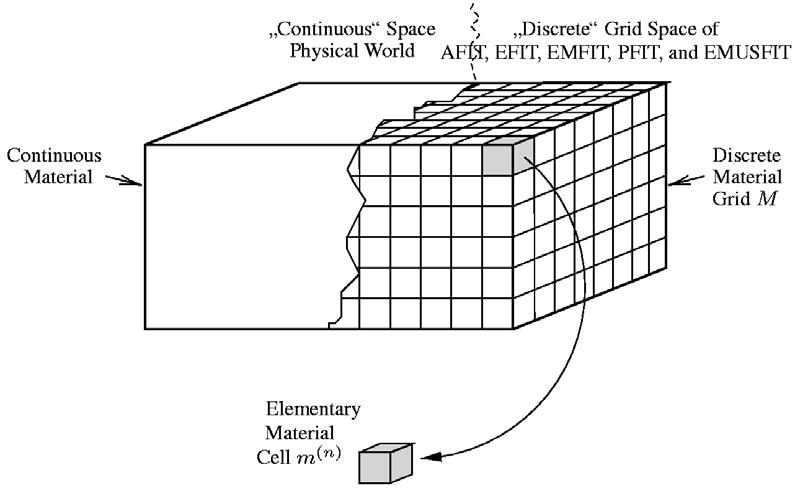
\includegraphics[width=0.8\textwidth]{bilder/discretization_material}
\caption{A discretization of the material in elementary material cells m, defining the material grid M.}
\label{fig:discretization_material}
\end{figure}


